\documentclass[twoside,twocolumn]{article}

\usepackage{blindtext} % Package to generate dummy text throughout this template 
\usepackage{graphicx}
\usepackage[sc]{mathpazo} % Use the Palatino font
\usepackage[T1]{fontenc} % Use 8-bit encoding that has 256 glyphs
\linespread{1.05} % Line spacing - Palatino needs more space between lines
\usepackage{microtype} % Slightly tweak font spacing for aesthetics

\usepackage[english]{babel} % Language hyphenation and typographical rules

\usepackage[hmarginratio=1:1,top=32mm,columnsep=20pt]{geometry} % Document margins
\usepackage[hang, small,labelfont=bf,up,textfont=it,up]{caption} % Custom captions under/above floats in tables or figures
\usepackage{booktabs} % Horizontal rules in tables

\usepackage{lettrine} % The lettrine is the first enlarged letter at the beginning of the text

\usepackage{enumitem} % Customized lists
\setlist[itemize]{noitemsep} % Make itemize lists more compact

\usepackage{abstract} % Allows abstract customization
\renewcommand{\abstractnamefont}{\normalfont\bfseries} % Set the "Abstract" text to bold
\renewcommand{\abstracttextfont}{\normalfont\small\itshape} % Set the abstract itself to small italic text

\usepackage{titlesec} % Allows customization of titles
\renewcommand\thesection{\Roman{section}} % Roman numerals for the sections
\renewcommand\thesubsection{\roman{subsection}} % roman numerals for subsections
\titleformat{\section}[block]{\large\scshape\centering}{\thesection.}{1em}{} % Change the look of the section titles
\titleformat{\subsection}[block]{\large}{\thesubsection.}{1em}{} % Change the look of the section titles

\usepackage{fancyhdr} % Headers and footers
\pagestyle{fancy} % All pages have headers and footers
\fancyhead{} % Blank out the default header
\fancyfoot{} % Blank out the default footer
\fancyhead[C]{Virtualizacion y contenedores $\bullet$ Mayo 2019 $\bullet$ } % Custom header text
\fancyfoot[RO,LE]{\thepage} % Custom footer text

\usepackage{titling} % Customizing the title section

\usepackage{hyperref} % For hyperlinks in the PDF

%----------------------------------------------------------------------------------------
%	TITLE SECTION
%----------------------------------------------------------------------------------------

\setlength{\droptitle}{-4\baselineskip} % Move the title up

\pretitle{\begin{center}\Huge\bfseries} % Article title formatting
\posttitle{\end{center}} % Article title closing formatting
\title{Patrones de Diseño} % Article title
\author{Yofer Nain Catari Cabrera}
\date{\today} % Leave empty to omit a date
\renewcommand{\maketitlehookd}{%
\begin{abstract}
\noindent Los patrones de diseño son soluciones típicas a problemas que ocurren comúnmente en el diseño de software. Son como planos prefabricados que puede personalizar para resolver un problema de diseño recurrente en su código.

No puede simplemente buscar un patrón y copiarlo en su programa, como puede hacerlo con las funciones o bibliotecas disponibles en el mercado. El patrón no es un código específico, sino un concepto general para resolver un problema en particular. Puede seguir los detalles del patrón e implementar una solución que se adapte a las realidades de su propio programa.

Los patrones a menudo se confunden con algoritmos, porque ambos conceptos describen soluciones típicas a algunos problemas conocidos. Si bien un algoritmo siempre define un conjunto claro de acciones que pueden lograr algún objetivo, un patrón es una descripción de más alto nivel de una solución. El código del mismo patrón aplicado a dos programas diferentes puede ser diferente.
\end{abstract}
}

%----------------------------------------------------------------------------------------

\begin{document}

% Print the title
\maketitle

%----------------------------------------------------------------------------------------
%	ARTICLE CONTENTS
%----------------------------------------------------------------------------------------

\section{Introduccion}

\lettrine[nindent=0em,lines=3]{L}a mayoría de los patrones se describen de manera muy formal para que las personas puedan reproducirlos en muchos contextos. Estas son las secciones que suelen estar presentes en una descripción de patrón:

La intención del patrón describe brevemente tanto el problema como la solución.
La motivación explica además el problema y la solución que el patrón hace posible.
La estructura de clases muestra cada parte del patrón y cómo están relacionadas.
El ejemplo de código en uno de los lenguajes de programación populares hace que sea más fácil captar la idea detrás del patrón.
Algunos catálogos de patrones enumeran otros detalles útiles, como la aplicabilidad del patrón, los pasos de implementación y las relaciones con otros patrones.



%------------------------------------------------

\section{Objetivos}

\begin{itemize}
\item  Los patrones son soluciones típicas a problemas comunes en el diseño orientado a objetos. Cuando una solución se repite una y otra vez en varios proyectos, alguien finalmente le pone un nombre y describe la solución en detalle. .
\item ...............................................



\end{itemize}




%------------------------------------------------

\section{Desarrollo}

\subsection{¿.................................?}

...................................................................................

\begin{center}
	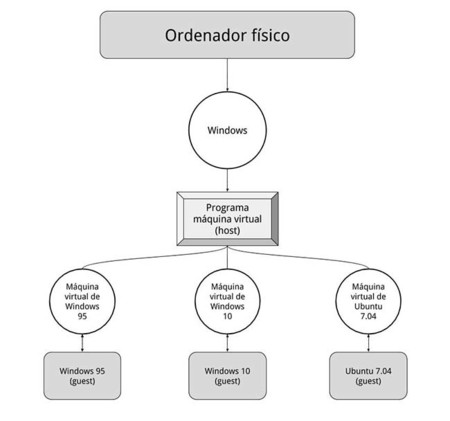
\includegraphics[width=5cm]{./Imagenes/virtualizacion} 
	\end{center}




\subsection{¿........................?}

........................................................................\\
........................................................................\\
...........................................................................

\begin{itemize}
\item .....................................
\\ -------------------------------------------------------------
\\.......
\\-------------------------------------------------------------------------------------------
\\ \textbf{-........................................................}


\begin{center}
	
\includegraphics[width=5cm]{./Imagenes/docker} 
	\end{center}

Ventajas
\\ \textbf{- .......................................................}
 

Desventajas
\\ \textbf{- .......................................................}
\end{itemize} 

\subsection{----------------------------------------------------?}
------------------------------------------------------------------

\begin{itemize}
	\item .....................................................
	\\ \textbf{-App} .......................................
	\\ \textbf{-App} .....................................
	\begin{center}
	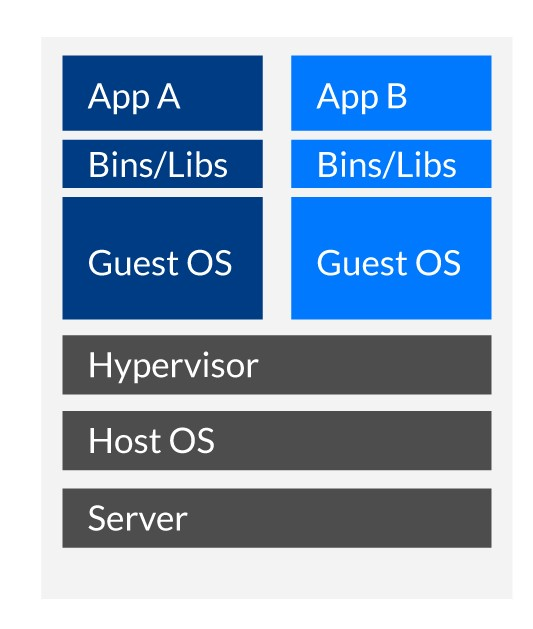
\includegraphics[width=5cm]{./Imagenes/jerarquia1} 
	\end{center}
\end{itemize} 

\begin{itemize}
	\item ..................................
.
	\\ \textbf{-App} .....................................
	\begin{center}
	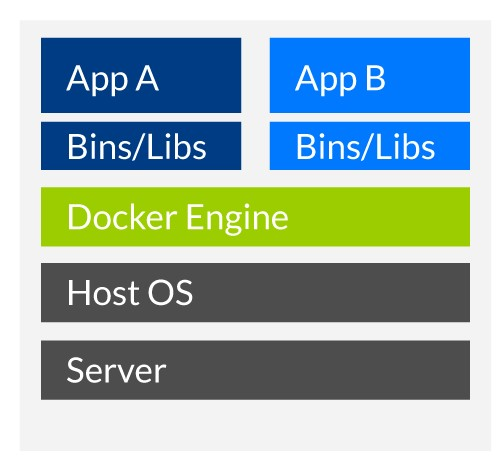
\includegraphics[width=5cm]{./Imagenes/jerarquia2} 
	\end{center}
\end{itemize} 

\begin{itemize}
	\item -------------------------------------------------------------------
		\item -------------------------------------------------------------------
			\item -------------------------------------------------------------------
	\item -------------------------------------------------------------------



\end{itemize} 

\section{Conclusiones}

---------------------------------------------------------------------------------.
%----------------------------------------------------------------------------------------
%	REFERENCE LIST
%----------------------------------------------------------------------------------------

\begin{thebibliography}{99} % Bibliography - this is intentionally simple in this template

\bibitem[Martin, 2011]{Diego Martin:2011dg}
Martin, M.M,  y J.U (2011).
\newblock Virtualización, una solución para la eficiencia,
seguridad y administración de intranets
\newblock {\em El profesional de la informacion}, 350.
\newblock Contenedor de aplicaciones: Docker (2015)
 
 
\end{thebibliography}

%----------------------------------------------------------------------------------------

\end{document}
